\section{Background and Design Considerations}
\label{sect:background}

Figure~\ref{fig:collocated} illustrates a converged IaaS cloud architecture 
where
each commodity server hosts a number of virtual machines and storage of these servers
is clustered using a distributed file system~\cite{googlefs03,hdfs10}.
Each physical machine hosts multiple virtual machines.  Every virtual machine
runs its own guest operating system and accesses virtual hard disks 
stored as image files maintained by the operating system running on the
physical host. 
%The secondary storage can be cluster-based and implemented with a distributed file system~\cite{googlefs03}.   
For VM snapshot backup, file-level semantics are normally not provided.
Snapshot operations take place at the virtual device driver level, which
means no fine-grained file system metadata can be used to determine the changed data. 
In a converged setting with source-side deduplication, the resources that are used to implement snapshot
backup and deduplication are the same resources that must support cloud-hosted
VMs.  Thus the backup service collocated with 
other cloud services has to minimize its resource impact.  
%This architecture does not use a separate  backup facility for a lower cost and 
%reduces the network bandwidth consumption in transferring the raw data for backup. 
%A backup service may co-locate with other cloud services on these commodity servers and 
%stores deduplicated data  in  the storage in this cluster or in
%a separate storage cluster.


%runs a backup service and 


%As discussed earlier, co-locating a backup service on the existing
%cloud cluster avoids the extra cost to acquire a dedicated backup facility

\begin{figure}[htb]
    \centering
    %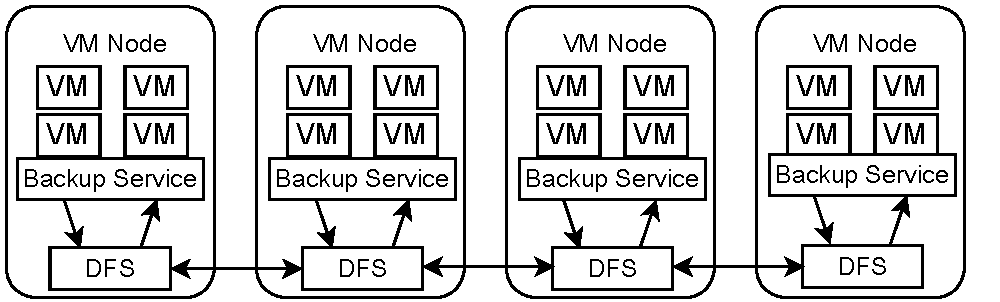
\includegraphics[width=3in]{images/colocated-arch}
    %\includegraphics[width=3in]{images/converged_arch}
    \resizebox{0.85\linewidth}{!}{
        %converged architecture diagram with a disrtibuted dedupe service, and secondary storage
\begin{tikzpicture}[thick,rounded corners,scale=0.8]\sf
	\definecolor{dfs}{gray}{0.90}
    %CDFS is the corner of the drawing (cluster with distributed file system)
    \coordinate (CDFS) at (0,0);
    %first we loop to draw 4 machines (and 4 VMs inside each machine)
    \foreach \x / \i in {0 / -1.5, 2.5 / -0.5, 5 / 0.5,8.0 / 1.5} {
        %CMAC is the coord of the current cluster machine
        \coordinate (CMAC) at ([xshift=\x cm]CDFS);
        %first draw the box around the machine
        \draw[-stealth] (CMAC) rectangle +(2.3,3) 
        %then the dots in the middle to represent more vms
        node[pos=0.5,anchor=south]{\scriptsize\ldots}
        %next the label centered near the top
        +(1.15,2.7) node[anchor=center]{\scriptsize{}Cluster Machine};
        %++(1.15,0) -- (4.9,-0.7);
        \draw[-stealth] ($(CMAC)+(1.15,0)$) -- ($(4.9,-0.7)+0.5*(\i,0)$);
        %now loop through the 4 vms we will draw
        \foreach \vmx in {0.1, 1.3} \foreach \vmy in {1,1.7} {
            \coordinate (CVM) at ([xshift=\vmx cm,yshift=\vmy cm]CMAC);
            %first draw the vm rectangle
            \draw[rounded corners=0.1cm] (CVM) rectangle +(0.8,0.6)
            %then draw a label node in the middle of it
            %the nodes is 50% along the line between the last two points
            %  (i.e. the diagonal of the rectangle)
            node[pos=0.5]{VM};
        }
    }
	\node at ([xshift=7.67cm,yshift=1.75cm,align=center,anchor=center]CDFS) {$\cdots$} ;
    %now we draw the distrubuted files systems across the VMs
    \draw[fill=dfs] ([xshift=0.1cm,yshift=0.1cm]CDFS) rectangle +(10.1,0.8) node[midway]
    {Source-side deduplication};
    \draw[fill=dfs] ([xshift=2.1cm,yshift=-1.5cm]CDFS) rectangle +(6.1,0.8) node[midway]
    {Secondary Storage};
\end{tikzpicture}

        %\includegraphics{figures/converged_arch}
    }
    \caption{VM snapshot backup running on a converged cloud cluster.}
    \label{fig:collocated}
\end{figure}

File backup systems have been developed to use fingerprints generated for
data ``chunks''  to identify duplicate
content~\cite{venti02,Rhea2008}.  In a simple implementation,
it is expensive to compare a large number of 
fingerprints
so a number of techniques have been proposed to improve duplicate identification. 
For example, the data domain method ~\cite{bottleneck08} 
uses an in-memory Bloom filter to identify non-duplicates and a prefetching cache for potential
duplicates that might hit in the future.
%An improvement to this work with parallelization is in ~\cite{MAD210,DEBAR}.
%Approximation techniques are studied in~\cite{extreme_binning09,Guo2011,WeiZhangIEEE}  
%to reduce memory requirements at the cost of some loss of deduplication
%efficiency.
Additional inline deduplication and  approximation techniques
are studied in ~\cite{extreme_binning09,sparseindex09,Srinivasan2012,WeiZhangIEEE}.  
%and a parallel batch solution for cluster-based deduplication is 
%studied in ~\cite{WeiZhangIEEE}. 
% \comments{
% All of the above approaches have focused on optimization of deduplication
% efficiency or speed, and none of them have considered the impact
% of deduplication on fault resilience in a cloud environment.  To do so, we
% examine the following properties of VM snapshot deduplication for converged
% IaaS architectures.
% }
%considered in this paper.
%Our consideration is discussed below.
%VM dependence minimization during deduplication and file system block management.

Even with these optimization and approximation techniques, resource usage such as memory  for deduplication
is still extensive for a shared cloud cluster.  
For example, in the experiments discussed in Section~\ref{sect:evaldedup}, 
the raw snapshot data has a size of 1,000TB on 100 physical machines that host VMs,
cross-machine fingerprint comparison using Bloom filter and approximated routing~\cite{bottleneck08,Dong2011} 
still needs several gigabytes of memory per machine. This can impact other primary cloud services sharing the same
computing resource. Our objective is to have an approximation scheme 
which uses no more than a few hundred megabytes of memory during normal operation.
Thus the  desired ratio of raw data to memory ratio is from 100K:1 to 30K:1.
Our proposed scheme achieves 85K:1
and this ratio is about the same as the number of machines increases.

Index sampling with a prefetch cache  is proposed 
in~\cite{Guo2011} for efficient single-machine deduplication. 
This scheme uses 25GB memory per 500TB of raw data
and thus the raw data to memory ratio is 20K:1. The scheme proposed in this paper 
uses three times less memory. We have not incorporated this index 
sampling technique because it is difficult to extend 
for a distributed architecture.  To use a distributed memory version 
of the sampled index, every deduplication
request may access a remote machine for index lookup and the overall overhead 
of access latency for all requests is significant.

% \comments{
% For example, the
% sampled index with prefetching, proposed  by Guo and Efstathopoulos\cite{Guo2011},
% uses 5GB memory space for 100TB of raw data even the compressed data size
% is about 5TB. It is fairly typical for
% a physical machine with terabytes of disk storage and tens of gigabytes of memory
% to support  more than 20 VMs and 10 snapshots per VM and can require  over 100TB of raw space
% even the actual storage space need is about 5TB assuming 20:1 compression ratio with deduplication.
% It is not easy  to adopt the sampled index method  for a distributed architecture
% and every deduplication request may access a remote machine for index lookup and the overall overhead of access latency
% for all requests can be significant.
%  In general
% with a cluster of machines in a cloud cluster, there will be more memory requirement per machine such as a
% fingerprint cache, for cross-machine fingerprint comparison~\cite{bottleneck08,Dong2011} and a deduplication
% task often needs several gigabytpes of memory, which impacts other cloud services sharing the computing resource.
% }

While deduplication reduces storage cost, it creates an artificial data dependence among VMs: when a shared data chunk
is lost in the storage, all VMs that refer such chunks after deduplication face a data loss.
The work in ~\cite{Reliability06} identifies such an issue in file systems 
and uses more replication for data shared by more files,
and we follow this idea and study VM-centric strategies.
When the backup storage is implemented using a distributed file system such as Hadoop and 
Google file system~\cite{googlefs03},  
the file system block  size is often chosen to be large (e.g. 64MB). On the other hand, 
deduplication implementations~\cite{Guo2011,extreme_binning09,bottleneck08,Jin2009,Dong2011}
 typically use smaller chunk sizes (e.g. 4K bytes).
Thus we need to address  the size gap between file system blocks and chunks.  
%in adding more replications for popular chunks. 

%Another disadvantage of cross-VM sharing is that it complicates
\comments{
Snapshot deletion 
%which is the garbage collection in VM environment
occurs frequently because snapshots expire regularly
and reference counting is required to identify chunks that are no loner used.
%Several well developed garbage collection methods do not apply to the
%converged virtualized architecture due to various environment and resource limitations:
Grouped mark-and-sweep~\cite{Guo2011} is effective for deletion by tracking
the dependencies from data containers to metadata groups, but still it carries
a significant cost in a cloud cluster. This is because any data chunk can still be
used by a large number of VMs, and there are multiple rounds of extensive I/O involved
to scan through the meta data of snapshots to check if a chunk is referenced or not.
As the number of machines increases, the I/O cost becomes more expensive.
% and  we show  such that only a subset of
%metadata needs to be scanned in order to reclaim the garbage in any given data container.
%However, data in VM environment tend to be highly dedupable which means
%such dependency could be extensive, therefore scanning a large subset of metadata still carries a significant cost,
% especially in a distributed setting.
Perfect hashing~\cite{Fabiano2013} provides a memory efficient way to represent a large set of
hashes in a compact form, however, it still requires the scanning of all data hashes before any 
garbage collection could begin, which limits its application to an offline batch process. 
In addition, it requires a centralized location
to store the hashing result which is still too big to be held in a converged architecture.

Our previous work on parallel deduplication~\cite{WeiZhangIEEE}
demonstrates the simulation results for  
is not a comprehensive VM-centric solution and does not address  snapshot deletion and file system block 
packaging for fault tolerance.  

Our previous work on popularity distribution of  deduplication~\cite{WeiZhangIEEE}
demonstrates the simulation results for  
The work in ~\cite{zhangusenix13} is a low-cost
solution, but requires all backups for each day to occur at the same time and is less flexible than the approach presented here.
}

\comments{
Our previous work on parallel deduplication~\cite{zhangusenix13} is a low-cost
solution, but it is not an inline solution and th backup for all VMs needs to be conducted
around the same time. 
It does not address  snapshot deletion and file system block packaging for fault tolerance. 

}


% a low cost solution, but it not an inline solution and 
%the backup for all VMs needs to be conducted
%around the same time. 

%Cross-VM chunk sharing also complicates 
% Snapshot deletion occurs frequently since  snapshots expire regularly
% and reference counting is required to identify chunks that are no longer used.
% The grouped mark-and-sweep approach~\cite{Guo2011}
% is effective for deletion, but still carries a significant cost, especially in a distributed
% setting.   This is because any data chunk can be used by any snapshot
% of virtual machines in a large cloud cluster and there are multiple rounds of  extensive I/O involved
% to scan through the metadata of snapshots to determine if a chunk has been used or not.
% As the number of virtual  machines increases, the cost becomes even worse.
%~\cite{Guo2011,Fabiano2013}  
%to count if a data chunk is still shared by other snapshots. 


%still significant
%especailly for a distributed setting.


% \comments{
% \paragraph*{Local versus Global Deduplication} --
% If deduplication is implemented strictly in the storage system,
% a data chunk is compared with fingerprints collected from all VMs during
% the deduplication process, and only a small number of
% copies of duplicates are stored in the storage.  This sharing
% artificially creates hidden data dependencies among different VMs owned by
% different
% who
% contract for isolation
% by the IaaS cloud platform.  That is, the unit of failure visible to the cloud
% user is the VM, but the unit of sharing in a deduplicated data store is the
% data chunk.

% Indeed, the greater the deduplication efficiency, the less
% the data redundancy is maintained, and the greater the ``hidden'' data
% dependence between VMs that must be hosted as if they were physically isolated.
% Thus,
% restricting deduplication to be local to each VM (but across snapshots)
% aligns the units of storage with the isolation properties guaranteed by the
% cloud at the possible expense of storage efficiency.
% %Localizing the impact of deduplication can increase fault isolation and resilience.
% %Thus from the fault tolerance point of view,  duplicate sharing among multiple VMs is
% %discouraged.


% Additionally, storage efficient deduplication can be computationally expensive
% to implement in a distributed setting.  In particular, duplicate detection is
% logically a ``global'' operation over all data chunks
% under consideration.
% By localizing duplicate search, the computational requirements
% for deduplication can be reduced, because fewer chunks must be compared.
% Further, deduplication of VMs can easily be implemented in
% parallel.

% Another disadvantage of cross-VM sharing is that it complicates
% snapshot deletion, which occurs frequently because snapshots expire regularly.
% Several well developed garbage collection methods do not apply to the
% converged virtualized architecture due to various environment and resource limitations:
% Grouped mark-and-sweep~\cite{Guo2011} is an effective approach by tracking
% the dependencies from data containers to metadata groups, such that only a subset of
% metadata needs to be scanned in order to reclaim the garbage in any given data container.
% However, data in VM environment tend to be highly redundant which means
% such dependency could be extensive, therefore scanning a large subset of metadata still carries a significant cost,
%  especially in a distributed setting.
% Perfect hashing~\cite{Fabiano2013} provides a very memory efficient way to represent a large set of
% hashes in a compact form, however, it still requires the scan of all data hashes before any garbage could begin,
% which limits its application to only offline batch garbage collection. In addition, it requires a centralized location
% to store the hashing result which is still too big to be hold anywhere in a converged architecture.


% Another disadvantage of cross-VM sharing is that it complicates
% snapshot deletion, which occurs frequently because snapshots expire regularly.
% Several well developed garbage collection methods do not apply to the
% converged virtualized architecture due to various environment and resource limitations:
% Grouped mark-and-sweep~\cite{Guo2011} is an effective approach by tracking
% the dependencies from data containers to metadata groups, such that only a subset of
% metadata needs to be scanned in order to reclaim the garbage in any given data container.
% However, data in VM environment tend to be highly dedupable which means
% such dependency could be extensive, therefore scanning a large subset of metadata still carries a significant cost,
%  especially in a distributed setting.
% Perfect hashing~\cite{Fabiano2013} provides a very memory efficient way to represent a large set of
% hashes in a compact form, however, it still requires the scan of all data hashes before any garbage could begin,
% which limits its application to only offline batch garbage collection. In addition, it requires a centralized location
% to store the hashing result which is still too big to be hold anywhere in a converged architecture.

% %to count if a data chunk is still shared by other snapshots.

% Thus,
% localizing deduplication to the VM can align fault isolation properties and
% guarantees, improve the computational efficiency of snapshot maintenance, and
% simplify snapshot deletion over non-localized approaches at the possible
% expense of storage efficiency.

% %minimize data sharing and simplify deletion while sacrificing
% %deduplication efficiency, and  can facilitate parallel execution of snapshot operations.
% \paragraph*{Units of Storage versus Units of Sharing} --
% The file system block  size in a distributed file system such as
% the Hadoop file system and the Google file system~\cite{googlefs03}
% is large (e.g.  64MB) so as to optimize file system performance
% for big data.
% Typically, deduplication implementations use smaller block sizes (4K bytes to
% 8K bytes on average~\cite{Jin2009}).
% In addition to the failure correlation that cross-VM data deduplication can
% introduce, disk block sharing of data chunks is another potential source of
% hidden data dependence.
% Thus a VM-centric solution should consider how data chunks from VMs are
% distributed among large file system blocks when a large-scale distributed file
% system is used for snapshot storage.

% %a minimum association of FSBs to VMs in the packaging
% %process. By minimizing this association we can improve fault tolerance by
% %reducing the number of VMs affected when storage nodes are lost.


% \paragraph*{Moderating Resource Usage} --
% In a converged setting, the resources that are used to implement snapshot
% backup and deduplication are the same resources that must support cloud-hosted
% VMs.  Thus the backup service must share the resources available to
% other cloud services as illustrated in Figure~\ref{fig:collocated},
% and has to minimize its impact on user-deliverable performance.
% %The key resource for global comparison  is memory for storing the fingerprints.
% %During snapshot deletion, reference counting for all unique blocks used in all VMs requires a significant resource usage
% %too.  Thus we seek for the low-profile techniques with approximation and low resource consumption.

% }

% \comments{
% With the above  considerations in mind, we propose a
% VM-centric approach (called VC)
% for a co-located backup service that has a resource usage profile
% suitable for use with converged cloud architectures.
% This compares the traditional deduplication approach {\em VM-oblivious} (VO)
% which manages duplicate data chunks without consideration of VMs.
% We discuss our key ideas and design in the next section.
% %Our key idea is to simplify deduplication management and
% }
% \comments{
% In designing a VC deduplication solution, we have considered and adopted some of
% the following previously-developed techniques.
% 1) {\em Changed Block Tracking}.
% VM snapshots can be  backed up  incrementally by identifying data segments that have
% changed from the previous version of the snapshot~\cite{Clements2009,Vrable2009,TanIPDPS2011}.
% Such a scheme  is  VM-centric since deduplication is localized to the snapshot
% history for each VM.
% %We are seeking for a tradeoff since
% %global signature comparison can deliver additional compression~\cite{Guo2011,Dong2011,extreme_binning09}.
% 1) {\em Stateless  Data Routing}.
% One approach to scalable duplicate comparison is to use content-based hash
% partitioning called stateless data routing by Dong et al.~\cite{Dong2011}.
% Stateless data routing divides the deduplication work with a similarity approximation. This work
% is similar to Extreme Binning by Bhagwat et al.~\cite{extreme_binning09} and
% each request is routed  to a machine which holds
% a Bloom filter  or can fetch on-disk index for additional comparison.
% While this approach is VM-oblivious, it motivates us to  use  a combined signature of a dataset to narrow
% VM-specific local search.
% 3) {\em Sampled Index for Memory Parsimony}.
% One effective approach that reduces memory usage is
% to use a sampled index with prefetching, proposed  by Guo and Efstathopoulos\cite{Guo2011}.
% The algorithm is VM oblivious and it is not easy  to adopt for a distributed architecture.
% To use a distributed memory version of the sampled index, every deduplication request
% may access a remote machine for index lookup and the overall overhead of access latency for all requests
% can be significant.

% We will first discuss and analyze the integration of the VM-centric deduplication strategies with fault isolation
% and discuss snapshot deletion support, then present an implementation design.
% }
